\documentclass{article}

\usepackage[spanish]{babel}
\usepackage{wrapfig}
\usepackage{amsmath}
\usepackage{graphicx}
\usepackage[colorlinks=true, allcolors=blue]{hyperref}

\begin{document}
\begin{titlepage}
        \begin{figure}
            \vspace{-8 em}
            \hspace{-10 em}
            
\includegraphics[width=5cm]{ipn} \hfill 
\includegraphics[width=4cm]{escom}
            \hspace{-8 em}
        \end{figure}
        \begin{center}
            {\large Instituto Politécnico Nacional \par}
            {\Large Escuela Superior de Cómputo \par}
            \vspace{3cm}
            {\scshape\Huge Práctica 5:\\ \bfseries Algoritmos Greedy \par}
            \vspace{3cm}
            {\itshape\Large Análisis de algoritmos \par}
            {\itshape\Large 3CV12 \par}
            \vfill
            {\Large Reyes Rodríguez Enrique Abdiel \par}
            {\Large Chávez Hernández Juan Diego \par}
            \vfill
            {\ \textit{abykings1@gmail.com} \par}
            {\ \textit{jdiegohdez0233@gmail.com} \par}
            \vfill
            {\Large Noviembre 2021\par}
        \end{center}
    \end{titlepage}
\newpage

    \textbf{Resumen: }
     En el siguiente trabajo se presenta el análisis a problemas cuya solución implementada es por medio de un algoritmo voraz, también llamado Greedy. Se realizarán los análisis a priori y a posteriori de un problema, con el fin de juzgar su uso.\\
    \textbf{Palabras clave: } Algoritmo, complejidad, greedy, huffmann.
\section{Introducción}
   Muchas veces, al intentar resolver un problema, se necesita proveer de una solución rápida. Aquí es donde entran en juego este tipo de algoritmo, cuya desventaja es que no siempre nos da soluciones correctas, ya que confían en las soluciones anteriores; por lo cual hay problemas que no se pueden resolver con este paradigma.\\
   Como ventaja es que son fáciles de implementar y ayudan a resolver problemas de optimización.  \\
   En la práctica se implementa la solución a un problema usando este paradigma, con el objetivo de mostrar el análisis de la complejidad temporal de un algoritmo tipo greedy.
    Como objetivo de la práctica está el demostrar el análisis de la complejidad temporal de un algoritmo tipo greedy.\cite{1}
\section{Conceptos básicos}
    Algoritmo voraz (\textbf{Greedy})\\
    Es un paradigma de programación en el que se basa en la idea de siempre buscar el mejor caso en cada paso que analiza. 
    Se comienza analizando a un conjunto de elementos que es del cual sale la solución,  por cada iteración, se realiza la selección y se agrega al conjunto solución.\cite{2}\\
    \\
    Codificación de \textbf{Huffmann}\\
    Algoritmo propuesto por David Huffmann, que se centra en la compresión de símbolos. Se basa en la asignación de un valor binario a cada símbolo de la entrada, y dadas las veces que aparece, es la longitud de el valor binario asociado. Se crea un árbol priorizando la longitud corta a niveles mas altos y la longitud larga a niveles mas bajos; por lo cual, los símbolos de salida son reducidos.\cite{3}\\
    \\
    Problema de la \textbf{Mochila Fraccionaria}\\
    Es un problema clásico en la implementación de algoritmos voraces. Este plantea que tenemos una mochila que puede cargar un peso  P y que tenemos n objetos fraccionables con un peso pi y un valor vi. Se trata de cargar la mochila sin pasarnos del peso máximo y maximizando el valor total seleccionando un objeto de cada clase en fracciones.Podemos no seleccionar un objeto, seleccionarlo o tomar una fracción.\cite{4}
    
    \newpage
 
    \textbf{Pseudocódigo implementado para el problema}
        \begin{verbatim}
            function fertilizante(d,r)
                s = {}
                f = r
                for i = 0, i<d.length , i**
                    if(i == 0 or i+1 == d.length) 
                        s.push(d[i])
                        f = r + d[i]
                    else
                        if (d[i]<f)
                            s.push(d[i])
                            f = r + d[i]
                return s
        \end{verbatim}
        \newpage
\section{Experimentación y resultados}
    \subsection{Problema del fertilizante}
    En este caso, se implementó una solucion voraz. Se observa que tiene un orden lineal, dado el rango del unico for que contiene, cuyo rango es el tamaño de el arreglo de entrada; En el cuerpo de este, sólo hay instrucciones de orden constante, por lo tanto, se tiene que $T(n) \in O(n)$
    \begin{figure}[h!]
        \centering
        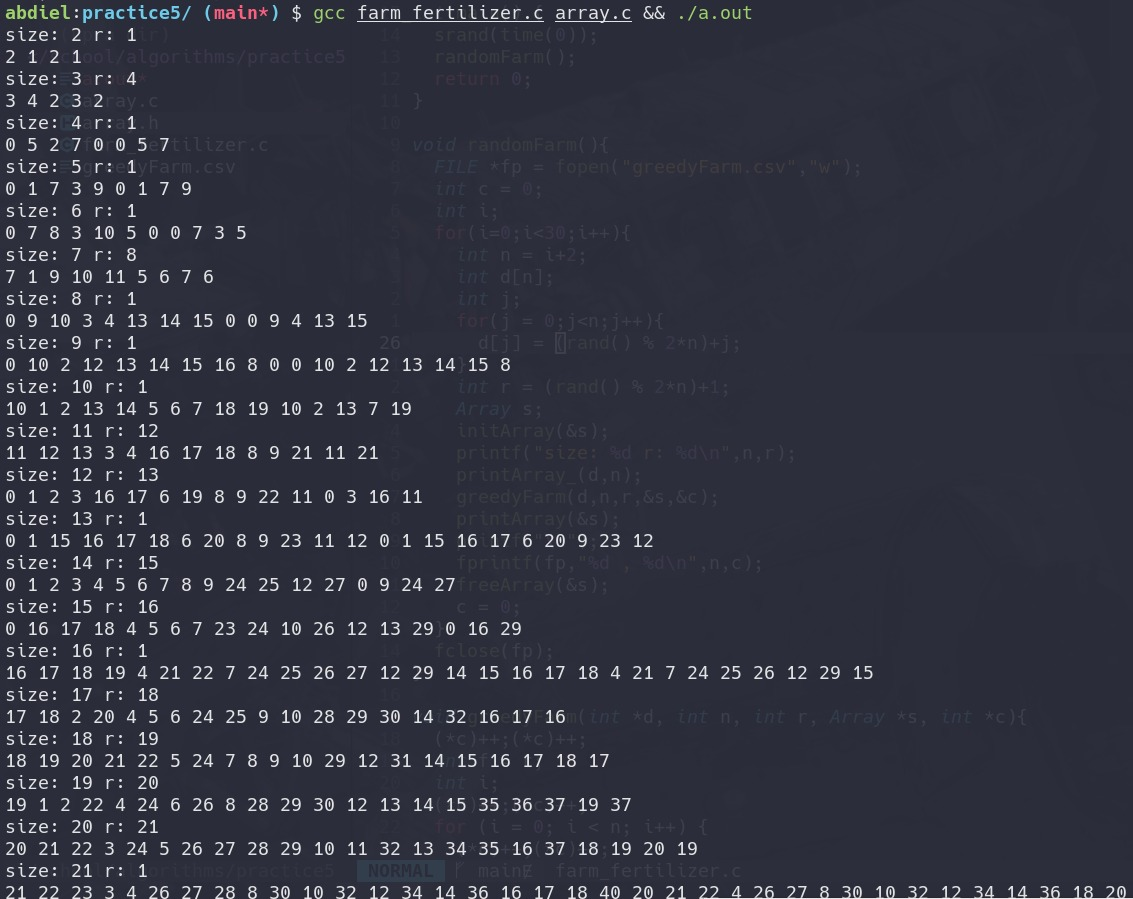
\includegraphics[width=0.9\textwidth]{greedy_console_out.jpeg}
        \caption{Esta es la compilacion y ejecucion de codigo en consola, donde a cada paso, se generan datos aleatorios}
        \label{fig:my_label}
    \end{figure}
    \newpage
    \begin{table}[h!]
            \centering
            \begin{tabular}{| c | c |}
            \hline
            n  & c   \\
            \hline
            2  & 16  \\
            3  & 20  \\
            4  & 28  \\
            5  & 32  \\
            6  & 38  \\
            7  & 36  \\
            8  & 48  \\
            9  & 58  \\
            10 & 54  \\
            11 & 52  \\
            12 & 60  \\
            13 & 76  \\
            14 & 68  \\
            15 & 70  \\
            16 & 92  \\
            17 & 76  \\
            18 & 80  \\
            19 & 84  \\
            20 & 88  \\
            21 & 118 \\
            22 & 96  \\
            23 & 132 \\
            24 & 104 \\
            25 & 108 \\
            26 & 144 \\
            27 & 116 \\
            28 & 152 \\
            29 & 134 \\
            30 & 162 \\
            31 & 136 \\
            \hline
            \end{tabular}
            \caption{Estos son los resultados de la ejecución del programa. En la primer columna, tenemos el tamaño del arreglo con el cual se ejecutó, va del 2 al 31. En la segunda columna tenemos el valor del contador, que muestra el numero de instrucciones ejecutadas. Se observa como el crecimiento es constante}
        \end{table}
        \newpage
        
        \begin{figure}[h!]
            \centering
            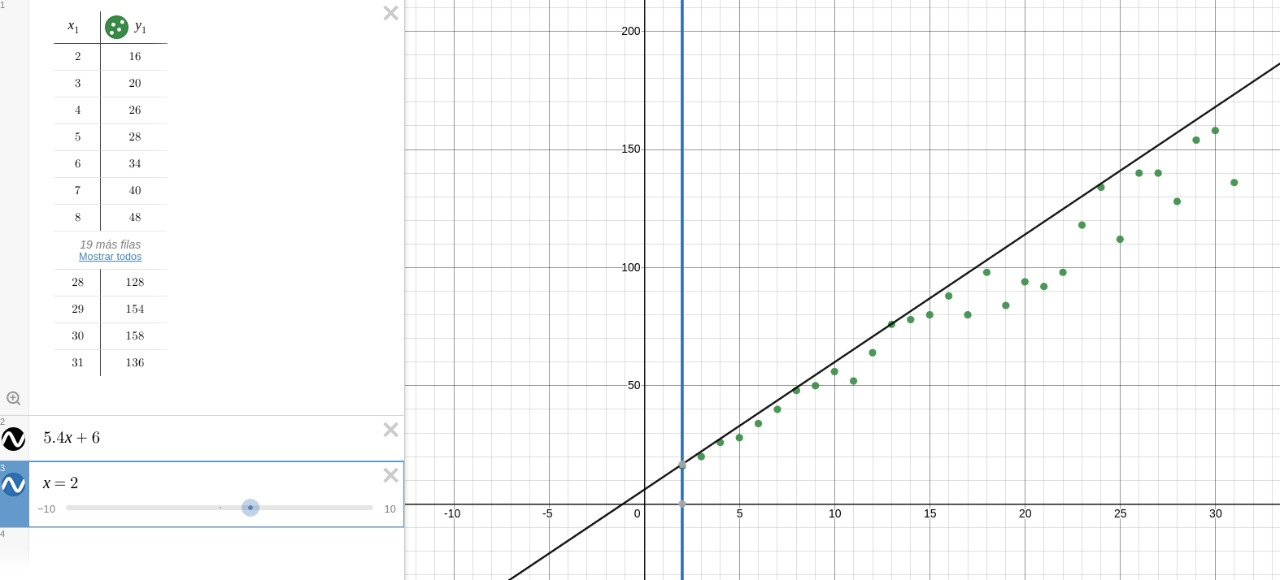
\includegraphics[width=0.9\textwidth]{greedy_graph.jpeg}
            \caption{Esta es la gráfica que obtenemos de la tabla anterior. Los puntos son las coordenadas dadas por la tabla, la recta negra es la función $y=5.4x+6$ obtenida ajustando la ecuación de la recta y $n0$ está en el punto $(2,0)$}
            \label{fig:my_label}
        \end{figure}
   
        
        
    
\newpage
\section{Conclusiones}
    \begin{wrapfigure}{l}{0in}
        \centering
        
\includegraphics[scale=0.2]{abdiel.png}
    \end{wrapfigure}
    Enrique Abdiel Reyes Rodríguez:\\
    Creo que este paradigma es muy útil para dar soluciones muy rápidas de implementar, aunque se tiene que ser muy cuidadoso con la parte que selecciona el valor óptimo local, ya que de eso depende la eficacia de la solución. Lo difícil fue entender el problema, ya que no se entendía lo que se pedía. Creo que el algoritmo provisto es una buena opción a elegir, pero hay más metodos que podrían ayudar a dar soluciones más competentes.\\
    
    \begin{wrapfigure}{r}{0in}
        \centering
        
\includegraphics[scale=0.2]{diego.jpg}
    \end{wrapfigure}
    Juan Diego Chávez Hernández:\\
    En el desarrollo de la práctica podemos observar que el uso de apuntadores es fundamental para poder generar soluciones del ejercicio, dichos apuntadores ayudaron al conteo de los pasos, y sobre todo para la implementación de un array dinámico, que fue muy útil para el conjunto solución. Cabe mencionar que en el ejercicio se realiza el análisis a posteriori y se comprueba que es lineal. Pienso que seria interesante encontrar una solución más óptima, pero no logramos encontrar alguna.\\
    \newpage
    \newpage
\section{Anexo}
    \subsection{Análisis a priori del algoritmo utilizado }
    Por medio del análisis por bloques de código vamos analizando el orden de complejidad de adentro hacia afuera. Empezamos por dentro del for, y vemos que todas sus instrucciones son constantes, por lo cual queda $O(n*1) = O(n)$. Las instrucciones del nivel superior también son constantes, realizamos la misma operación $O(n*1) = O(n)$.\\Vemos que para este caso, se tiene que $T(n) \in O(n)$\\
    \textbf{Pseudocódigo implementado para el problema}
        \begin{verbatim}
            function fertilizante(d,r)
                s = {} O(1)----|
                f = r  O(1)--------------------|
                for i = 0, i<d.length , i**------------------------O(n)
                    if(i == 0 or i+1 == d.length) O(1)-----O(1)--|
                        s.push(d[i])     O(1)-------!      |
                        f = r + d[i]     O(1)-------!      |
                    else                                   |
                        if (d[i]<f) -------------- O(1)----|
                            s.push(d[i]) O(1)-------|
                            f = r + d[i] O(1)-----|
                return s
        \end{verbatim}\\
    \subsection{Preguntas}
    \textbf{¿Cuál sería la mejor función de selección voraz en el caso en el que todos los objetos tuvieran el mismo valor?}\\
    Ordenando los objetos conforme al peso y seleccionando los que son más ligeros, así se guarda el máximo de objetos en la mochila.\\
    \textbf{¿Cuál sería la mejor función de selección voraz en el caso en el que todos los objetos tuvieran el mismo peso?}\\
    Entonces se tienen que seleccionar los objetos de mayor valor, ordenándolos y escogiéndolos conforme al mayor valor hasta que la mochila llegue a la máxima capacidad.\\
    \newpage
    \textbf{Mostrar mediante un contra ejemplo, que al elegir objetos enteros, el algoritmo greedy no encuentra soluciones óptimas}\\
    Sea $W={8,7,6,5,4,3,2,1}$\\
    Sea $V={10,9,8,7,6,5,4,3}$\\
    Los valores en la mochila irian hasta:\\
    $V={0,3,7,12}$\\
    $W={9,3,6,3}$\\
    Al siguiente paso, la solución óptima estaría dada por la fracción $v/w = 6/4$ dándonos\\
    $V={0,3,7,12,16.5}$\\
    $W={9,3,6,3,0}$\\
    Pero al no poder partir el objeto, nos quedamos sin objetos para elegir, quedándonos un valor total menor.
    
    \textbf{Construir la codificación de Huffmann para la cadena: ciencias de la tierra}\\
    0011111000000001111101011011000011001100111010111001111111100010010101\\
     \begin{figure}[h!]
        \centering
        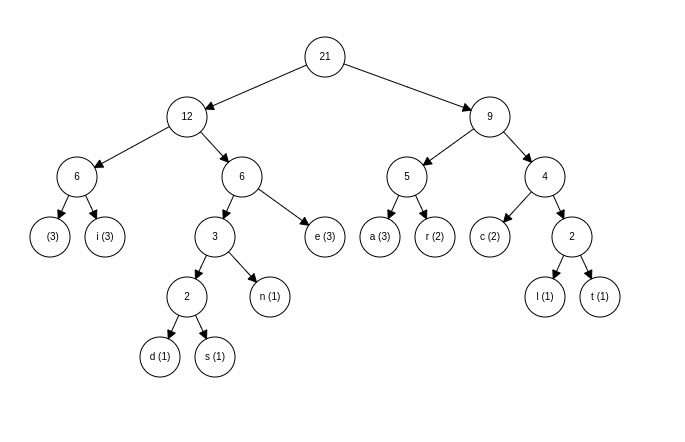
\includegraphics[width=0.9\textwidth]{huffmann_tree.jpeg}
        \caption{Este es el árbol obtenido a partir de la cola de prioridad, donde se observa la frecuencia de cada caracter}
        \label{fig:my_label}
    \end{figure}
    
    \textbf{Documentar el orden de complejidad del algoritmo de Huffmann}\\
    Durante la codificación de caracteres a bits, la cola de prioridad juega un papel fundamental en crear el arbol y es la parte de mayor orden en el algoritmo; al ir asignando el peso en el arbol se tiene una $O(nlogn)$ para irse moviendo en el arbol e insertarlo. 
    \newpage
    \begin{figure}[h!]
        \centering
        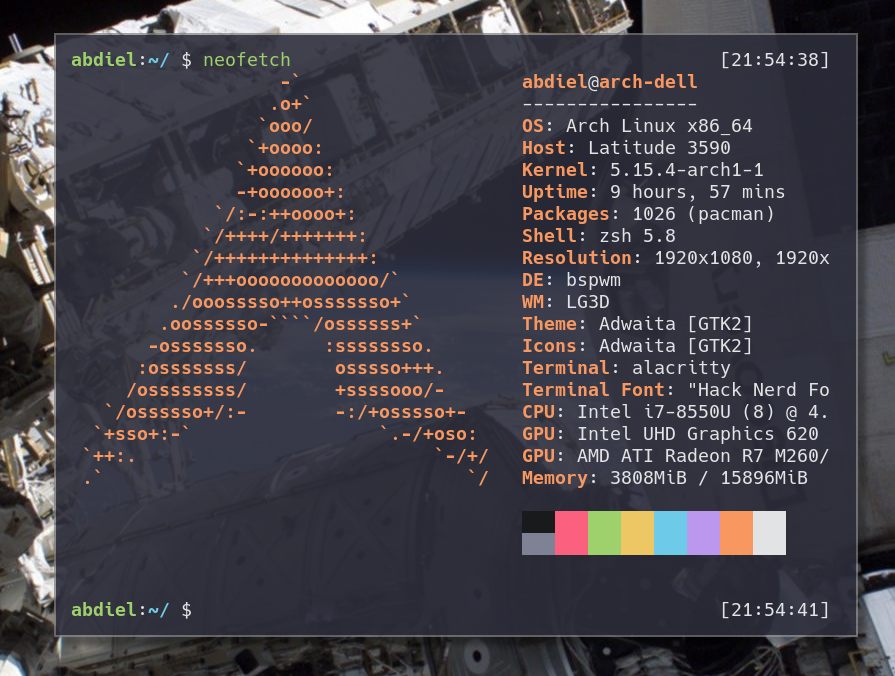
\includegraphics[width=0.9\textwidth]{specs.png}
        \caption{Estas son las especificaciones de la máquina en donde se ejecutó}
        \label{fig:my_label}
    \end{figure}
\newpage    
        
\begin{thebibliography}{}
    
        \bibitem{1}Cormen, T. H., Leiserson, C. E., Rivest, R. L., & Stein, C. (2009). Introduction to algorithms. MIT press.
        \bibitem{2}Algoritmos Voraces | Aprende Programación Competitiva. (s. f.). Olimpiada de Informatica. Recuperado 26 de noviembre de 2021, de https://aprende.olimpiada-informatica.org/algoritmia-voraz
        \bibitem{3}Huffman. (s. f.). UMA. Recuperado 26 de noviembre de 2021, de https://neo.lcc.uma.es/evirtual/cdd/tutorial/presentacion/huffman.html
        \bibitem{4}GeeksforGeeks. (2021, 24 noviembre). 0-1 Knapsack Problem | DP-10. https://www.geeksforgeeks.org/0-1-knapsack-problem-dp-10/
    \end{thebibliography}

\end{document}